\documentclass[11pt]{article}
\usepackage[utf8]{inputenc}
\usepackage[T1]{fontenc}
\usepackage[letterpaper]{geometry}
\geometry{verbose,tmargin=1.5cm,bmargin=1.5cm,lmargin=1.5cm,rmargin=1.5cm,columnsep=0.8cm}
\usepackage[english]{babel}
\usepackage{graphicx}
\usepackage{longtable}
\usepackage{float}
\usepackage{fouriernc}
\usepackage{amssymb}
\usepackage{hyperref}
\usepackage{framed}
\tolerance=1000
\usepackage{enumitem}
\usepackage{multicol}

\usepackage{tikz}
\usetikzlibrary{arrows,automata,positioning,fit,shapes}
 
\begin{document}

\begin{center}
\huge EECE7398 --- Compilers

Assignment 5

\vskip1cm

\normalsize\ttfamily Bruno S M M Morais <soutomaiormunizmo.b@husky.neu.edu>

All code can be found on \url{https://github.com/brunosmmm/eece7398}

\end{center}

\vskip1cm

\section*{Question 1}
\subsection*{item (a)}

\begin{figure}[H]
\centering

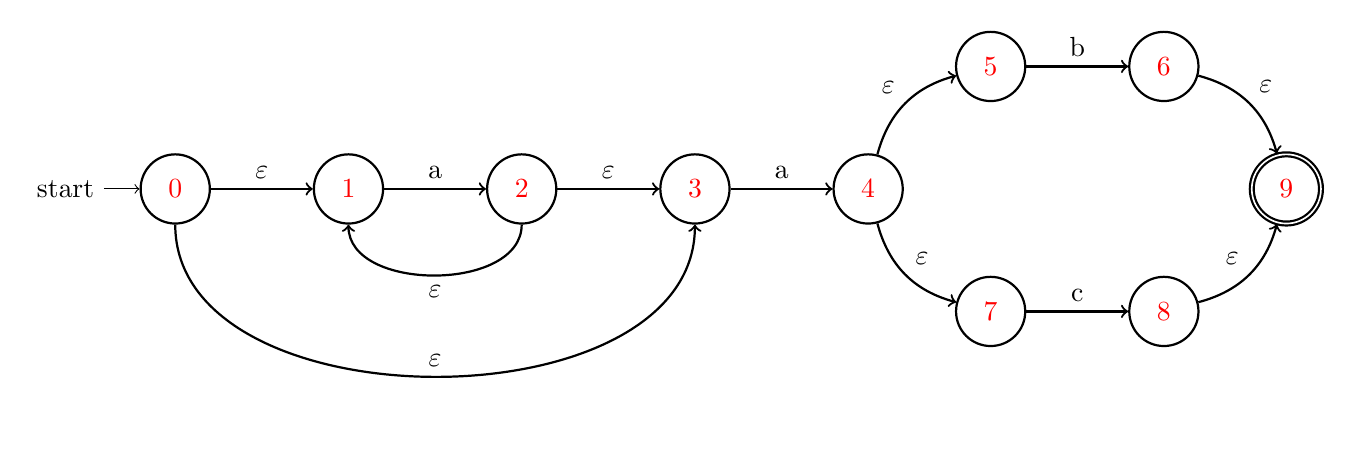
\begin{tikzpicture}[auto,node distance = 2.2cm]

\tikzstyle{every state}=[thick,fill=none,draw=black,text=red]
\tikzstyle{nfabound}=[draw=blue,rounded corners,dashed]

%a*
\node [state,initial] (s0) {0};
\node [state] (s1) [right of=s0] {1};
\node [state] (s2) [right of=s1] {2};
\node [state] (s3) [right of=s2] {3};

\path [->,thick] (s0) edge node {$\varepsilon$} (s1)
      [->,thick] (s1) edge node {a} (s2)
      [->,thick] (s2) edge node {$\varepsilon$} (s3)
      [->,thick] (s2) edge [bend left,out=90,in=90] node {$\varepsilon$} (s1)
      [->,thick] (s0) edge [bend left, out=270, in=270] node {$\varepsilon$} (s3);

%a(b|c)
\node [state] (s4) [right of=s3] {4};
\node [state] (s5) [above right of=s4] {5};
\node [state] (s6) [right of=s5] {6};
\node [state] (s7) [below right of=s4] {7};
\node [state] (s8) [right of=s7] {8};
\node [state,accepting] (s9) [below right of=s6] {9};

\path [->,thick] (s3) edge node {a} (s4)
      [->,thick] (s4) edge [bend left] node {$\varepsilon$} (s5)
      [->,thick] (s4) edge [bend right] node {$\varepsilon$} (s7)
      [->,thick] (s5) edge node {b} (s6)
      [->,thick] (s7) edge node {c} (s8)
      [->,thick] (s6) edge [bend left] node {$\varepsilon$} (s9)
      [->,thick] (s8) edge [bend right] node {$\varepsilon$} (s9);

\end{tikzpicture}
\caption{NFA for regular expression a*a(b|c)}
\end{figure}

\subsection*{item (b)}

Converting to a DFA:

\begin{itemize}

\item Initial state $q_{0} = \{0\} \Rightarrow \varepsilon-closure(\{0\}) = \{0, 1, 3\}$ 

\item From A with ``a'' we reach the states \{2,4\}. $\varepsilon-closure \left(MOVE\left( \{2,4\}, a \right) \right) = \{1,3,5,7\}$.

\item Similarly, for ``b'' and ``c'' in state B we determine that the final state C is reached.

\end{itemize}

\begin{table}[H]
\centering
\begin{tabular}{c c c c c}
$S_{NFA}$ & $s_{DFA}$ & a & b & c \\
\hline
\{\textcolor{red}{0},\textcolor{red}{1},\textcolor{red}{3}\}  & A        & B & --- & --- \\
\{\textcolor{red}{1},\textcolor{red}{3},\textcolor{red}{5},\textcolor{red}{7}\}& B        & B & C   & C   \\
\{\textcolor{red}{9}\}      & C        & --- & --- & --- \\
\hline  
\end{tabular}
\caption{State transition table}
\end{table}

\begin{figure}[H]
\centering
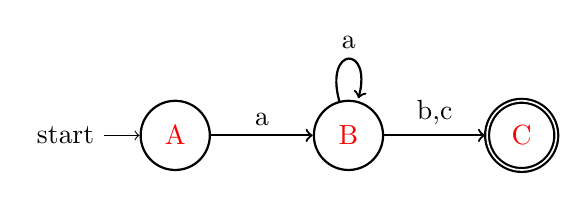
\begin{tikzpicture}[auto,node distance = 2.2cm]

\tikzstyle{every state}=[thick,fill=none,draw=black,text=red]
\tikzstyle{nfabound}=[draw=blue,rounded corners,dashed]

\node [state,initial] (A) {A};
\node [state] (B) [right of=A] {B};
\node [state,accepting] (C) [right of=B] {C};

\path [->,thick] (A) edge node {a} (B)
      [->,thick] (B) edge [loop above] node {a} ()
      [->,thick] (B) edge node {b,c} (C);


\end{tikzpicture}
\caption{DFA resulting transition graph}
\end{figure}

\end{document}
